% =============================================================================
%  Data engineering report — Project 0: Ubisoft vs Electronic Arts (EN)
%  Build: latexmk -xelatex report-en.tex   (see README.md in this folder)
% =============================================================================
\documentclass[11pt, a4paper, oneside, headings=normal, numbers=noenddot, DIV=12]{scrartcl}
\usepackage[english]{babel}
\usepackage{steam-report}
\graphicspath{{../livraison/figures/en/}}
\sisetup{group-separator={,}, group-minimum-digits=4}

% --- Metadata ----------------------------------------------------------------
\newcommand{\ReportAuthor}{LUMU BAMANA MANASSE}
\newcommand{\ReportAuthorRole}{Data engineer}
\newcommand{\ReportShortTitle}{Ubisoft vs Electronic Arts · Data engineering report}
\newcommand{\ReportFooter}{October 2026 · v1.0.0}
\newcommand{\ReportKicker}{Data engineering report · Project 0}
\newcommand{\ReportTitle}{Ubisoft vs\\Electronic Arts}
\newcommand{\ReportSubtitle}{What Steam data reveals:\\an end-to-end ETL pipeline, from client brief to acceptance}
\newcommand{\ReportMeta}{%
  \begin{tabularx}{\linewidth}{@{}>{\bfseries}l@{\hspace{1em}}Y@{}}
  Date & October 2026 \\
  Version & 1.0.0 (delivered and accepted) \\
  Client & Lumen Forge Games (fictional) · Engagement LFG-2026-001 \\
  GitHub repository & \url{https://github.com/MediJr/ubisoft-vs-ea-steam-etl} \\
  Language & English · \textit{version française disponible dans le dépôt}
  \end{tabularx}}
\newcommand{\ReportScenario}{Fictional scenario, real data: the client and its staff are invented to simulate a complete professional
  engagement. The data comes from the public Steam and SteamSpy APIs, extracted on 21 October 2026.
  This project is not affiliated with Ubisoft, Electronic Arts or Valve.}
\hypersetup{pdftitle={Ubisoft vs Electronic Arts: data engineering report}, pdfauthor={Lumu Bamana Manasse},
  pdfsubject={Steam ETL pipeline, portfolio project}, pdflang={en-US}}

\begin{document}
\MakeTitlePage

% =============================================================================
\section*{Document control}
\addcontentsline{toc}{section}{Document control}

\begin{tabularx}{\linewidth}{@{}>{\bfseries\sffamily}L{4.2cm}Y@{}}
\toprule
Project & Portfolio project 0: ETL pipeline on public Steam data \\
Engagement & LFG-2026-001: ``Understand what works for major publishers on Steam'' \\
Client & Lumen Forge Games, independent studio based in Lyon, France (fictional), attn. Camille Roux \\
Author & Lumu Bamana Manasse, data engineer \\
Delivery period & October 2026 \\
Data & Extraction of 21 October 2026, 18:38 to 19:10 (Paris time) \\
Status & \pill{good}{DELIVERED} \pill{good}{ACCEPTED WITH MINOR RESERVATIONS} \\
Source code & \url{https://github.com/MediJr/ubisoft-vs-ea-steam-etl} \\
\bottomrule
\end{tabularx}

\subsection*{Version history}
\begin{tabularx}{\linewidth}{@{}l l Y@{}}
\toprule
\textbf{Version} & \textbf{Date} & \textbf{Description} \\
\midrule
0.1 & 2026-10-21 & Scoping: brief, meeting minutes, statement of work \\
0.9 & 2026-10-21 & Complete pipeline, analyses, data quality fixes \\
1.0.0 & 2026-10-22 & Acceptance testing, final report (French and English), publication \\
\bottomrule
\end{tabularx}

\subsection*{Reading guide}
\begin{tabularx}{\linewidth}{@{}>{\bfseries}L{4.2cm}Y@{}}
Decision maker (client) & \hyperref[sec:summary]{1. Executive summary} and \hyperref[sec:results]{11. Results and recommendations} \\
Data lead & 2. Scoping, 4. Architecture, 7. Data quality, 10. Acceptance, 12. Limitations \\
Engineer taking over & 5. Pipeline, 6. Data model, 9. Operations, appendices \\
\end{tabularx}

\begingroup
\addtokomafont{sectionentry}{\color{primary}}
\setcounter{tocdepth}{2}
\tableofcontents
\endgroup
\clearpage

% =============================================================================
\section{Executive summary}\label{sec:summary}

\textbf{The need.} Lumen Forge Games, an independent studio with no data team, is preparing to release its first game on Steam
at around €25. Before setting its price and launch strategy, it wants to learn what works (and what fails) for two major publishers:
\textbf{Ubisoft} and \textbf{Electronic Arts}.

\textbf{The solution.} A Python ETL pipeline automatically collects public data from Steam and SteamSpy (six sources), cleans it and
loads it into a DuckDB analytical database. Ten SQL queries answer the four business questions, and a report presents the findings.
Everything runs with \textbf{a single command}.

\kpirow{100}{games analysed\\(50 per publisher)}{9.8 M}{Steam reviews\\aggregated}{930}{raw API responses\\kept}{0}{personal data\\collected}
\kpirow{6}{data\\sources}{30 min}{full extraction\\(fresh clone)}{2 s}{batch replay\\with no API calls}{6 / 6}{acceptance criteria\\met}

\begin{keybox}[Key findings]
\begin{itemize}[leftmargin=1.2em]
  \item \textbf{Q1 · Satisfaction:} a tie on average (80\%), but two opposite profiles. EA is ``hit or miss''
        (85\% median, yet 11 games below 70\%). Ubisoft is more consistent, and its games \textbf{gain 3.2 points after release}.
  \item \textbf{Q2 · Price:} the more expensive a game, the lower its rating (correlation of about $-0.5$). Above €60, satisfaction drops.
  \item \textbf{Q3 · Longevity:} the games that last are free-to-play or multiplayer.
  \item \textbf{Q4 · French speakers:} slightly more generous (+2 points), but they write only 2\% of reviews.
\end{itemize}
\end{keybox}

\textbf{What this project demonstrates on the engineering side:} API-friendly extraction (throttling, retries, resume cache),
an immutable dated raw layer, transactional loading with no duplicates, privacy \emph{by design} (no player username is ever downloaded),
detection and correction of four data quality issues in real-world data, and a documented incident recovery.

% =============================================================================
\section{Context and scoping}

\subsection{From a vague request to measurable questions}
The initial request fit in one sentence: ``understand what works for the big publishers''. The scoping meeting turned it into four
questions, each tied to a concrete client decision.

\begin{table}[H]
\centering
\begin{tabularx}{\linewidth}{@{}l Y L{4.1cm}@{}}
\toprule
\textbf{\#} & \textbf{Business question} & \textbf{Decision supported} \\
\midrule
Q1 & Which of the two publishers best satisfies its players on Steam, and is that satisfaction stable over time? & Post-launch reputation monitoring \\
Q2 & Are more expensive games rated higher? Are discounts a sign of trouble? & Launch price and discount policy \\
Q3 & Which games keep their players years after release? & Post-launch content \\
Q4 & Do French-speaking players judge these publishers differently? & Priority market \\
\bottomrule
\end{tabularx}
\caption{Business questions agreed during scoping}
\end{table}

\subsection{Scope}
\begin{tabularx}{\linewidth}{@{}Y Y@{}}
\toprule
\textcolor{good}{\textbf{In scope}} & \textcolor{warn}{\textbf{Out of scope}} \\
\midrule
Games of type \texttt{game} published on Steam by Ubisoft or EA & DLC, soundtracks, demos, bundles \\
At least 500 reviews, at most 50 games per publisher (most reviewed) & Other platforms: EA app, Ubisoft Connect, consoles \\
Store pages, review summaries, monthly history, player counts & Review text and any personal data \\
Analysis report and re-runnable pipeline & Stock market impact, interactive dashboard, automated scheduling \\
\bottomrule
\end{tabularx}

\subsection{Approach}
The project follows the five phases of a data consulting engagement. Each phase produces deliverables versioned in the repository.

\begin{table}[H]
\centering\small
\begin{tabularx}{\linewidth}{@{}l L{3.2cm} Y@{}}
\toprule
\textbf{Phase} & \textbf{Purpose} & \textbf{Deliverables} \\
\midrule
1 & Scoping & Client brief, scoping minutes, statement of work (\texttt{docs/mission/}) \\
2 & Extraction & \texttt{src/extract.py}, raw layer \texttt{data/raw/}, ADR 002 \\
3 & Transformation and loading & \texttt{src/transform.py}, \texttt{src/load.py}, \texttt{sql/00\_schema.sql} \\
4 & Analysis & 10 SQL queries, 5 charts, auto-generated results \\
5 & Delivery & Acceptance (sign-off), this report, documentation, publication \\
\bottomrule
\end{tabularx}
\caption{Engagement phases}
\end{table}

% =============================================================================
\section{Data sources}

\begin{table}[H]
\centering\small
\begin{tabularx}{\linewidth}{@{}L{3.8cm} L{2.0cm} Y L{1.9cm}@{}}
\toprule
\textbf{Source} & \textbf{Status} & \textbf{Data used} & \textbf{Purpose} \\
\midrule
Steam Store search & Unofficial & List of a publisher's games (\texttt{app\_id}) & Scope \\
Store page (\texttt{appdetails}) & Public, undocumented & Publisher, price in euros, discount, genres, release date & Q2, Q3 \\
Reviews (\texttt{appreviews}) & Public, documented & Review totals, all languages and French & Q1, Q4 \\
History (\texttt{appreview\-histogram}) & Unofficial & Positive and negative reviews per month & Q1 \\
Steam Web API & Official & Concurrent players & Q3 \\
SteamSpy & Third party & Owner estimates, previous-day peak & Information \\
\bottomrule
\end{tabularx}
\caption{Source inventory}
\end{table}

\textbf{Constraints.} Steam tolerates about 200 requests per 5 minutes. Three endpoints are unofficial and may change without
notice. No API key is required, so there are no secrets to manage.

\begin{keybox}[Upfront exploration: test before committing]
Before signing the statement of work, every endpoint was tested by hand. The \texttt{day\_range} parameter of the reviews API
\emph{seems} to filter reviews over a period, but in fact it \textbf{does not change} the returned summary. Without that test, the
stability measure (Q1) would have been promised on a false premise. The monthly history (\texttt{appreviewhistogram}) is what made it possible.
\end{keybox}

% =============================================================================
\section{Solution architecture}

\begin{figure}[H]
\centering
\resizebox{\linewidth}{!}{%
\begin{tikzpicture}[
  font=\sffamily\small, node distance=0.5cm and 0.9cm,
  src/.style={draw=rule, fill=panel, rounded corners=2pt, minimum width=2.7cm, minimum height=0.75cm, align=center},
  stage/.style={draw=primary, fill=primary, text=white, rounded corners=3pt, minimum width=2.5cm, minimum height=1.3cm, align=center, font=\sffamily\small\bfseries},
  store/.style={cylinder, shape border rotate=90, aspect=0.18, draw=accent, fill=accent!8, minimum width=2.3cm, minimum height=1.5cm, align=center},
  deliv/.style={draw=accent, rounded corners=2pt, minimum width=2.6cm, minimum height=0.75cm, align=center},
  arr/.style={-{Stealth[length=2.6mm]}, thick, color=ink2}]
  \node[src] (s1) {Steam Store\\\scriptsize search + store pages};
  \node[src, below=of s1] (s2) {Steam reviews\\\scriptsize summary + history};
  \node[src, below=of s2] (s3) {Steam Web API\\\scriptsize concurrent players};
  \node[src, below=of s3] (s4) {SteamSpy\\\scriptsize estimates};
  \node[stage, right=1.2cm of $(s2.east)!0.5!(s3.east)$] (e) {EXTRACT\\\scriptsize\mdseries 2 passes · cache};
  \node[store, below=1.1cm of e] (raw) {\scriptsize data/raw/\\\scriptsize YYYY-MM-DD\\\scriptsize JSON + manifest};
  \node[stage, right=of e] (t) {TRANSFORM\\\scriptsize\mdseries scope · typing};
  \node[stage, right=of t] (l) {LOAD\\\scriptsize\mdseries transaction};
  \node[store, right=of l] (db) {\scriptsize DuckDB\\\scriptsize 5 tables};
  \node[deliv, right=1.1cm of db, yshift=1.1cm] (o1) {10 SQL queries};
  \node[deliv, below=0.35cm of o1] (o2) {5 charts};
  \node[deliv, below=0.35cm of o2] (o3) {Report + acceptance};
  \foreach \s in {s1,s2,s3,s4} \draw[arr] (\s.east) -- (e.west);
  \draw[arr] (e) -- node[right, font=\scriptsize\sffamily, text=ink2]{written as is} (raw);
  \draw[arr] (raw.east) -| (t.south);
  \draw[arr] (t) -- (l);
  \draw[arr] (l) -- (db);
  \foreach \o in {o1,o2,o3} \draw[arr] (db.east) -- (\o.west);
  \begin{scope}[on background layer]
    \node[draw=rule, dashed, rounded corners=6pt, fit=(e)(t)(l)(raw), inner sep=10pt, label={[font=\scriptsize\sffamily, text=ink2]above:python -m src.pipeline}] {};
  \end{scope}
\end{tikzpicture}}
\caption{Pipeline architecture: one command chains extraction, transformation, loading and report generation}
\end{figure}

\subsection{Technology choices}
\begin{table}[H]
\centering\small
\begin{tabularx}{\linewidth}{@{}L{2.5cm} L{3.4cm} Y@{}}
\toprule
\textbf{Need} & \textbf{Choice} & \textbf{Rationale and rejected alternatives} \\
\midrule
Language & Python 3.14 & Data engineering standard, rich ecosystem \\
HTTP calls & \texttt{requests} & Simple and reliable. \texttt{httpx} (async) is unnecessary at this volume. \\
Transformation & \texttt{pandas} & Fits a few thousand rows. Polars is faster but brings no gain here. \\
Storage & DuckDB (file) & Serverless analytical SQL. PostgreSQL will be the novelty of project 1. \\
Analysis & SQL & Readable, verifiable, independent from Python \\
Charts & \texttt{matplotlib} & Static figures embedded in the report \\
Environment & \texttt{venv} + \texttt{pip} & Universal. \texttt{uv} and Poetry come later. \\
Orchestration & None (one command) & Deliberate at level 0. Dagster is planned for project 3. \\
\bottomrule
\end{tabularx}
\caption{Technology stack (details: ADR 001)}
\end{table}

\subsection{Design principles}
\begin{enumerate}[leftmargin=1.4em]
  \item \textbf{Immutable raw layer:} API responses are stored unchanged. A transformation bug is fixed by replaying the batch,
        without calling the APIs again.
  \item \textbf{Idempotency:} running the pipeline twice gives the same result, with no duplicates (primary keys, full refresh).
  \item \textbf{Privacy by design:} personal data is never requested from the APIs.
  \item \textbf{Reproducibility:} every figure in this report comes from a versioned query. \texttt{resultats.md} is regenerated on every run.
  \item \textbf{Traceability:} one manifest per batch, an exclusions table with reasons, and three ADRs for the key decisions.
\end{enumerate}

% =============================================================================
\section{Pipeline design}

\subsection{Extraction}
Collecting all six sources for the 160 candidate games would have taken about 1,000 calls, more than 25 minutes, for games that
would partly be discarded anyway. Extraction therefore runs in \textbf{two passes}:

\begin{table}[H]
\centering\small
\begin{tabularx}{\linewidth}{@{}l Y r r@{}}
\toprule
\textbf{Step} & \textbf{Action} & \textbf{Ubisoft} & \textbf{EA} \\
\midrule
Discovery & Steam search by publisher, ``games'' category & 80 & 80 \\
Light pass & Review summary (1 call per game), ``at least 500 reviews'' filter & 77 & 76 \\
Detailed pass & 5 calls per selected game & 77 & 76 \\
\bottomrule
\end{tabularx}
\caption{Extraction funnel (batch of 2026-10-21)}
\end{table}

\textbf{Robustness.} Each call is preceded by a 1.5\,s pause. HTTP 429 (too many requests) and 5xx errors trigger up to three
retries with increasing back-off. An explicit \texttt{User-Agent} identifies the project. Every response is cached in the raw layer,
so an interrupted extraction resumes where it stopped. Writes are \textbf{atomic}, a change made after the incident described in
section~\ref{sec:incident}:

\begin{lstlisting}[language=Python]
temporary = path.with_suffix(".tmp")
temporary.write_text(json.dumps(payload, ensure_ascii=False, indent=2), encoding="utf-8")
temporary.replace(path)   # instant rename: never a half-written file
\end{lstlisting}

\textbf{Privacy at the source.} Reviews are requested with \texttt{num\_per\_page=0}: Steam returns totals only, with no individual
review, hence no username or identifier.

\subsection{Transformation}
\begin{table}[H]
\centering\small
\begin{tabularx}{\linewidth}{@{}L{3.4cm} Y@{}}
\toprule
\textbf{Rule} & \textbf{Implementation} \\
\midrule
Scope & Type \texttt{game}, already released, actual publisher matches the searched publisher \\
Cap & The 50 most reviewed games per publisher. The others are logged in \texttt{exclusions} (53 games). \\
Typing & French dates (``12 janv. 2023'') parsed to \texttt{DATE}, prices in euros, SteamSpy ranges to integers \\
Missing values & Review rate \texttt{NULL} rather than 0 when there are no reviews. A free game costs €0. \\
History & Unix timestamps converted to months, aggregated if Steam returns weekly buckets \\
\bottomrule
\end{tabularx}
\caption{Transformation rules}
\end{table}

\subsection{Loading}
Loading uses a \textbf{full refresh} strategy: the schema is recreated, then every table is inserted, \textbf{within a single
transaction}. On failure nothing is committed and the database keeps its previous state. It is never half-loaded.

\begin{lstlisting}[language=Python]
connection.execute("BEGIN TRANSACTION")
try:
    connection.execute(SCHEMA_PATH.read_text(encoding="utf-8"))
    for name in LOAD_ORDER:                      # games first (foreign keys)
        connection.register("incoming", tables[name])
        connection.execute(f"INSERT INTO {name} BY NAME SELECT * FROM incoming")
        connection.unregister("incoming")
    connection.execute("COMMIT")
except Exception:
    connection.execute("ROLLBACK")
    raise
\end{lstlisting}

% =============================================================================
\section{Data model}

\begin{figure}[H]
\centering
\resizebox{0.95\linewidth}{!}{%
\begin{tikzpicture}[font=\sffamily\scriptsize,
  ent/.style={draw=primary, fill=white, rounded corners=2pt, align=left, inner sep=5pt},
  rel/.style={-{Stealth[length=2mm]}, thick, color=accent}]
  \node[ent] (g) {\textbf{\normalsize games}\\[2pt]\textbf{app\_id} \textit{PK}\\name, publisher\_group\\price\_initial\_eur, discount\_percent\\steam\_release\_date, years\_on\_steam\\genres, metacritic\_score, \dots};
  \node[ent, left=1.6cm of g] (r) {\textbf{\normalsize review\_summary}\\[2pt]\textbf{app\_id, language} \textit{PK}\\total\_reviews, total\_positive\\positive\_rate};
  \node[ent, right=1.6cm of g] (m) {\textbf{\normalsize reviews\_monthly}\\[2pt]\textbf{app\_id, month} \textit{PK}\\reviews\_up, reviews\_down};
  \node[ent, below=1.2cm of g] (p) {\textbf{\normalsize player\_snapshot}\\[2pt]\textbf{app\_id, snapshot\_date} \textit{PK}\\current\_players\\peak\_players\_yesterday};
  \node[ent, dashed, draw=ink2, right=1.6cm of p] (x) {\textbf{\normalsize exclusions}\\[2pt]\textbf{app\_id, publisher\_searched} \textit{PK}\\reason};
  \draw[rel] (r) -- node[above]{2 per game} (g);
  \draw[rel] (m) -- node[above]{1 per month} (g);
  \draw[rel] (p) -- node[right]{1 per day} (g);
\end{tikzpicture}}
\caption{DuckDB data model (arrows represent foreign keys)}
\end{figure}

\begin{table}[H]
\centering\small
\begin{tabularx}{\linewidth}{@{}l Y r@{}}
\toprule
\textbf{Table} & \textbf{Grain (one row per…)} & \textbf{Rows} \\
\midrule
\texttt{games} & selected game & 100 \\
\texttt{review\_summary} & game and language (\texttt{all}, \texttt{french}) & 200 \\
\texttt{reviews\_monthly} & game and month & \num{9929} \\
\texttt{player\_snapshot} & game and extraction date & 100 \\
\texttt{exclusions} & discarded candidate, with its reason & 53 \\
\bottomrule
\end{tabularx}
\caption{Tables, grain and volumes (full data dictionary in appendix~\ref{app:dict})}
\end{table}

% =============================================================================
\section{Data quality}

\subsection{Built-in checks}
\begin{itemize}[leftmargin=1.2em]
  \item \textbf{Schema constraints:} primary keys, \texttt{NOT NULL}, foreign keys. An anomaly makes loading fail instead of skewing results.
  \item \textbf{Control query} (\texttt{sql/controle\_recette.sql}): no duplicates, volume per publisher, review threshold, no personal column.
  \item \textbf{Exclusions table:} every discarded candidate has a reason. Nothing disappears without a trace.
\end{itemize}

\subsection{Issues detected and fixed}
Real-world data revealed four issues that reading the API documentation alone could not have anticipated.

\begin{table}[H]
\centering\small
\begin{tabularx}{\linewidth}{@{}L{3.1cm} Y Y@{}}
\toprule
\textbf{Symptom} & \textbf{Cause} & \textbf{Fix} \\
\midrule
5 release dates not parsed & Steam writes ``aout'' (August) without its accent, and one page has no date & Month dictionary accepts both spellings. The missing date stays \texttt{NULL}. \\
\midrule
0 exclusions on first run: a result too perfect & Games dropped by the 50-game cap were not logged & 53 exclusions recorded with reasons \\
\midrule
Player peak of 0 for 9 recent games (\textit{Battlefield 6}: 0, vs.\ 45,100 online) & SteamSpy does not track them yet: 0 means ``unknown'' & Switched to the official Steam API (ADR 003) \\
\midrule
21 EA games ``launched'' in 2020 & EA returned to Steam in 2020, and some games predate Steam reviews & Q1b requires first reviews to match the Steam release date \\
\bottomrule
\end{tabularx}
\caption{Data quality issues found in real-world data}
\end{table}

\begin{keybox}[Lesson]
A zero is not always a zero, and a perfect result is suspicious. Data quality cannot be assumed: it must be verified,
dataset by dataset, before any analysis.
\end{keybox}

% =============================================================================
\section{Security, compliance and governance}

\begin{tabularx}{\linewidth}{@{}L{3.6cm} Y@{}}
\toprule
\textbf{Topic} & \textbf{Measure} \\
\midrule
Personal data (GDPR) & The reviews API can return usernames, identifiers and texts. Applying \textbf{data minimisation} (Art.~5(1)(c))
and \textbf{data protection by design} (Art.~25), only totals are requested. Verified: no \texttt{steamid} or \texttt{personaname}
field in the 930 raw files, and no personal column in the database. \\
Secrets & No API key required. The \texttt{.gitignore} still excludes any \texttt{.env} file. \\
Published data & Data is not versioned (\texttt{data/} is ignored): it is regenerated by the pipeline. \\
API usage & Deliberately throttled, explicit \texttt{User-Agent}, non-commercial use \\
Traceability & One manifest per batch, dated work log, ADRs, CHANGELOG \\
\bottomrule
\end{tabularx}

% =============================================================================
\section{Operations}

\subsection{Commands}
\begin{lstlisting}[language=bash]
python -m venv .venv && .venv\Scripts\activate     # isolated environment (Windows)
pip install -r requirements.txt
python -m src.pipeline                             # today's extraction + processing (~30 min)
python -m src.pipeline --run-date 2026-10-21       # replay a raw batch, no API calls (~2 s)
\end{lstlisting}

\subsection{Capture of a full run}
Actual log of the acceptance run on a fresh environment (timestamps and paths shortened, intermediate progress hidden;
the pipeline logs in French):

\begin{terminal}{PowerShell · python -m src.pipeline}
\begin{lstlisting}[style=terminal]
19:16:24 | INFO | src.extract   | Extraction vers ...\00-jeux-video-etl\data\raw\2026-10-21
19:16:29 | INFO | src.extract   | Ubisoft : 80 jeux candidats
19:19:17 | INFO | src.extract   | Ubisoft : 76 jeux avec au moins 500 avis
19:31:55 | INFO | src.extract   | Electronic Arts : 80 jeux candidats
19:34:39 | INFO | src.extract   | Electronic Arts : 76 jeux avec au moins 500 avis
19:46:47 | INFO | src.extract   | Extraction terminée
19:46:47 | INFO | src.transform | Table games            :    100 lignes
19:46:47 | INFO | src.transform | Table review_summary   :    200 lignes
19:46:47 | INFO | src.transform | Table reviews_monthly  :   9768 lignes
19:46:47 | INFO | src.transform | Table player_snapshot  :    100 lignes
19:46:47 | INFO | src.transform | Table exclusions       :     52 lignes
19:46:47 | INFO | src.load      | Base chargée : ...\data\steam.duckdb
19:46:49 | INFO | src.report    | Graphiques et résultats écrits dans ...\docs\livraison
19:46:49 | INFO | pipeline      | Pipeline terminé en 1825 s
\end{lstlisting}
\end{terminal}

\subsection{Incident and recovery}\label{sec:incident}
\begin{table}[H]
\centering\small
\begin{tabularx}{\linewidth}{@{}l Y@{}}
\toprule
\textbf{Time} & \textbf{Event} \\
\midrule
18:38 & Production extraction started \\
19:05 & \textbf{External interruption} of the process, at 56 of 76 EA games \\
19:06 & Diagnosis: no running process, no manifest, 133 games cached. Check: no truncated JSON file. \\
19:06 & Same command relaunched: the 133 cached games are re-read in \textbf{0.1\,s}, then collection resumes \\
19:10 & Extraction complete. Improvement: atomic writes, so that a hard stop can never leave a corrupted file. \\
\bottomrule
\end{tabularx}
\caption{Timeline of the 2026-10-21 incident}
\end{table}

% =============================================================================
\section{Testing and acceptance}

Acceptance testing was run on a \textbf{fresh environment}: a copy of the publishable files only (38 files, no data, no virtual
environment), a new Python environment, then the single command from the README.

\begin{table}[H]
\centering\small
\begin{tabularx}{\linewidth}{@{}l L{4.2cm} Y c@{}}
\toprule
\textbf{\#} & \textbf{Criterion} & \textbf{Result} & \\
\midrule
C1 & End-to-end run with one command & Install in 54\,s, pipeline in 30\,min 25\,s, exit code 0 & \ok \\
C2 & No duplicates after a re-run & Same volumes before and after: 100 / 200 / \num{9929} / 100 / 53 & \ok \\
C3 & At least 15 games per publisher & 50 games per publisher, all with at least 500 reviews (minimum: \num{7215}) & \ok \\
C4 & One query and one answer per question & 10 queries, one section per question & \ok \\
C5 & No personal data & No personal field in 930 raw files or in the database & \ok \\
C6 & Limitations stated & Section~\ref{sec:limits} & \ok \\
\bottomrule
\end{tabularx}
\caption{Acceptance results (details: \texttt{docs/livraison/2026-10-21-pv-recette.md}, in French)}
\end{table}

\begin{warnbox}[Minor reservations]
\textbf{R1 · Panel reproducibility.} Steam's search relevance order varies slightly between runs. Between production and acceptance,
99 of 100 games are identical. Key indicators match to one decimal place (weighted rates: EA 77.4\%, Ubisoft 81.3\%). \\
\textbf{R2 · Discounts.} No game was on sale on extraction day, so this part of Q2 cannot be answered.
\end{warnbox}

% =============================================================================
\section{Results and recommendations}\label{sec:results}

\subsection{Q1 · Who best satisfies its players, and for how long?}
\begin{figure}[H]
\centering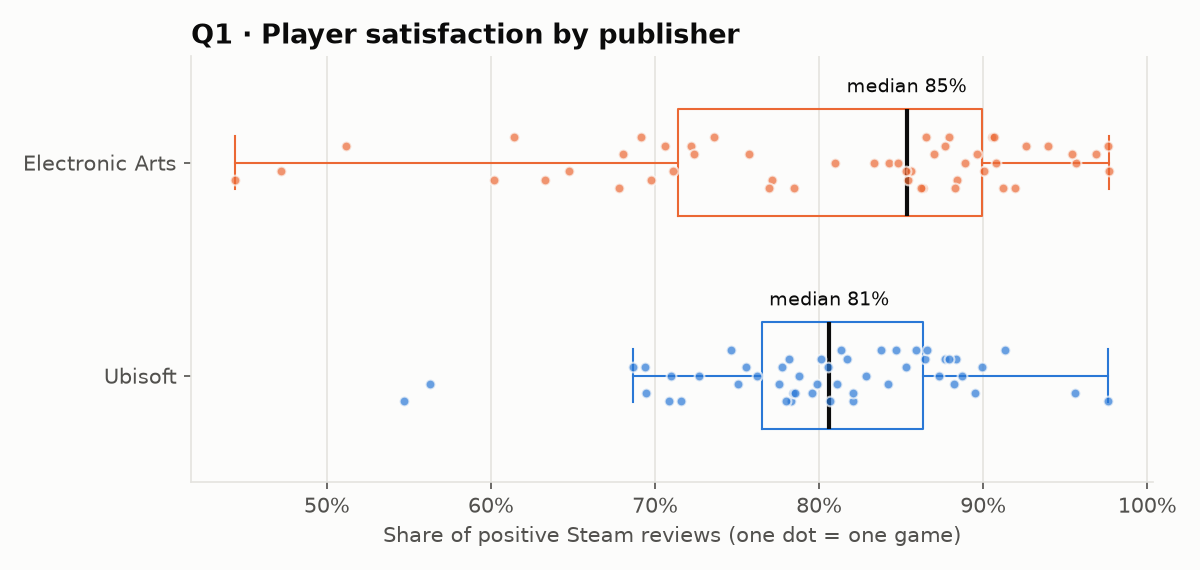
\includegraphics[width=0.92\linewidth]{q1_satisfaction_par_editeur.png}
\caption{Share of positive reviews per game and per publisher}
\end{figure}

\begin{table}[H]
\centering\small
\begin{tabularx}{\linewidth}{@{}Y r r r r r r@{}}
\toprule
\textbf{Publisher} & \textbf{Mean} & \textbf{Median} & \textbf{Weighted} & \textbf{< 70\%} & \textbf{Change} & \textbf{Recovered} \\
\midrule
\textbf{Electronic Arts} & 80.3\% & 85.3\% & 77.4\% & 11 & $-1.0$ pt & 4 / 34 \\
\textbf{Ubisoft} & 80.2\% & 80.6\% & 81.3\% & 5 & $+3.2$ pts & 12 / 39 \\
\bottomrule
\end{tabularx}
\caption{Overall satisfaction, then change between the first 3 months and the last 12 months on Steam}
\end{table}

A tie on average, but two profiles: EA is more spread out (higher median, but twice as many games below 70\%), whereas Ubisoft
is more consistent and \textbf{improves its games after release} (\textit{Assassin's Creed Unity} +24.5 points, \textit{The Crew 2} +25.5).

\begin{figure}[H]
\centering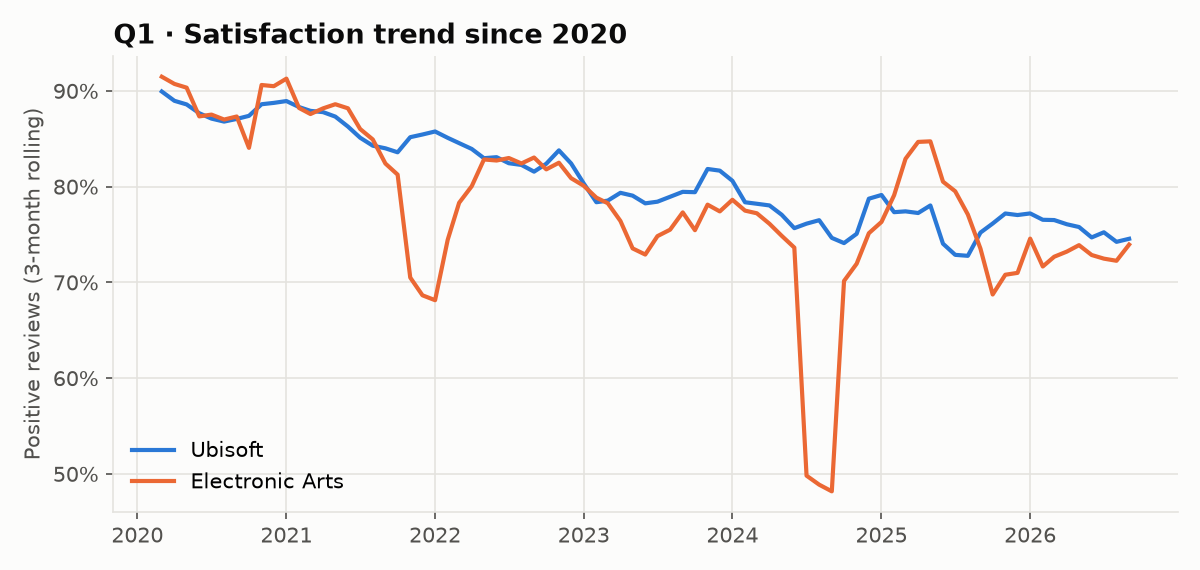
\includegraphics[width=0.92\linewidth]{q1_evolution_mensuelle.png}
\caption{Monthly trend: two visible crises at EA}
\end{figure}

The monthly history reveals two crises at EA: the launch of \textit{Battlefield 2042} (November 2021: \num{40065} negative reviews,
35\% positive, since recovered by +30.7 points), and a \emph{review bombing} of \textit{Apex Legends} in July 2024
(\num{82120} negative reviews in one month, 7\% positive), six years after its release.

\subsection{Q2 · Are more expensive games rated higher?}
\begin{figure}[H]
\centering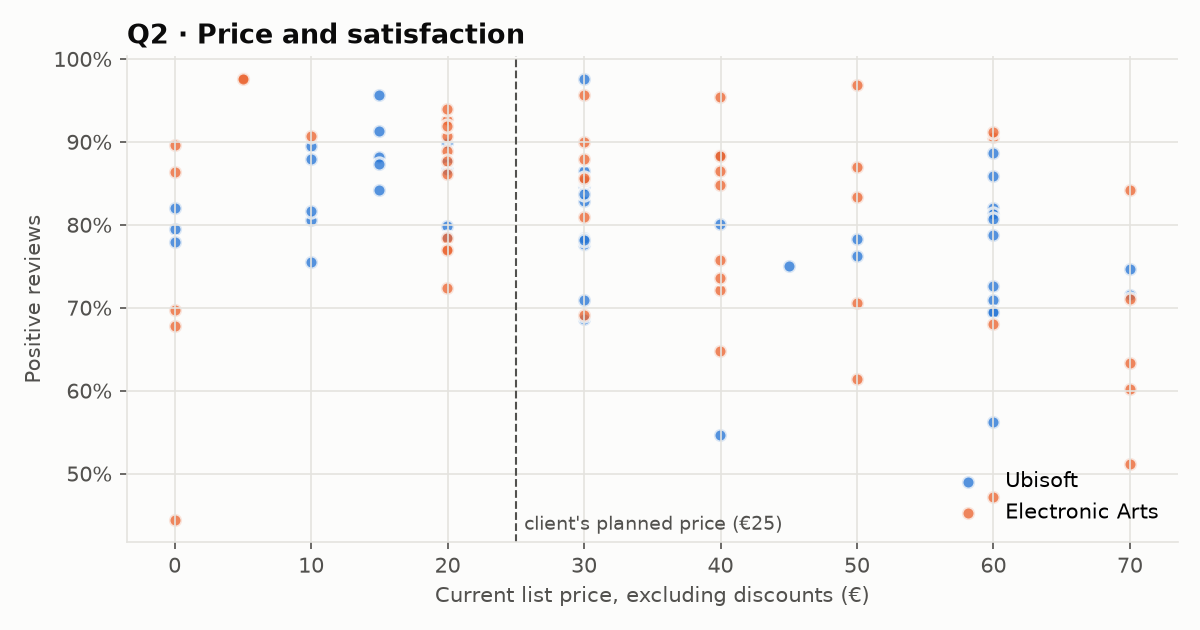
\includegraphics[width=0.88\linewidth]{q2_prix_satisfaction.png}
\caption{Current list price and satisfaction}
\end{figure}

No, rather the opposite: the correlation is $-0.55$ for EA and $-0.46$ for Ubisoft (Spearman: $-0.49$ for both). At €60 and above,
the median drops to 63\% (EA) and 73\% (Ubisoft). The €20--40 band, where the client sits, ranges from 80 to 86\%. Since the price is the
\emph{current} list price, \textbf{survivorship bias} is possible: older, cheap games that still sell are often classics.

\subsection{Q3 · Which games keep their players?}
\begin{figure}[H]
\centering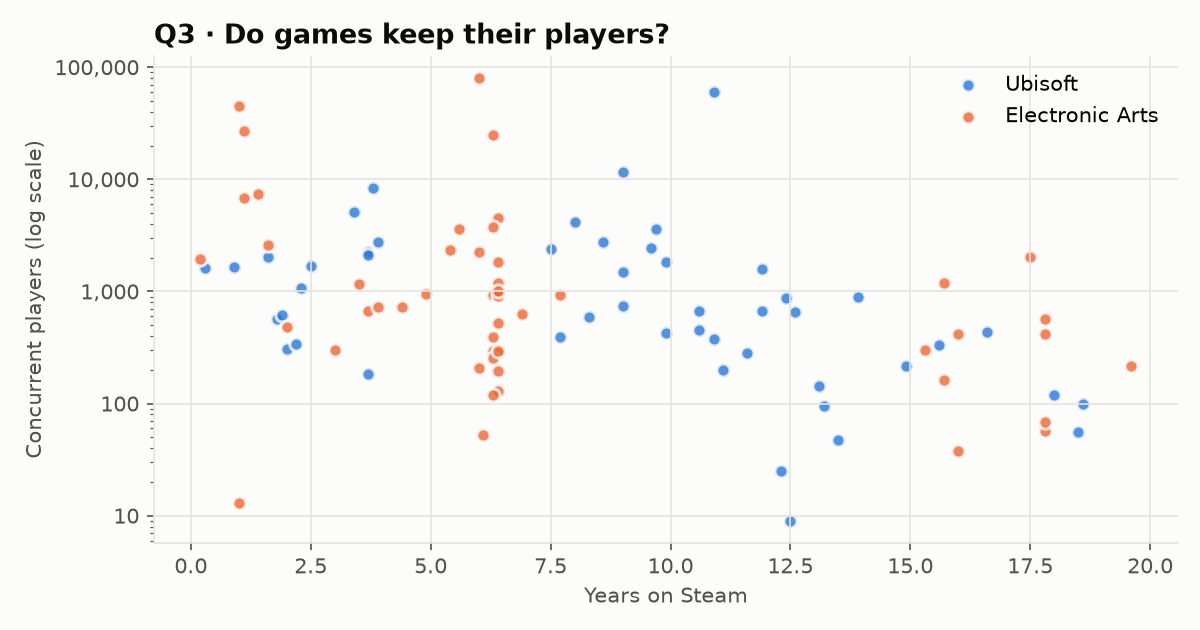
\includegraphics[width=0.88\linewidth]{q3_longevite.png}
\caption{Years on Steam and concurrent players (log scale)}
\end{figure}

The four most-played games aged 5 years or more are \textbf{free-to-play}: \textit{Apex Legends} (\num{79893} concurrent players),
\textit{Rainbow Six Siege} (\num{60193}), \textit{The Sims 4} and \textit{Brawlhalla}. Among paid games, multiplayer, co-op
(\textit{It Takes Two}, 95\% positive) and large role-playing games are the ones that last.

\subsection{Q4 · Do French-speaking players judge differently?}
\begin{figure}[H]
\centering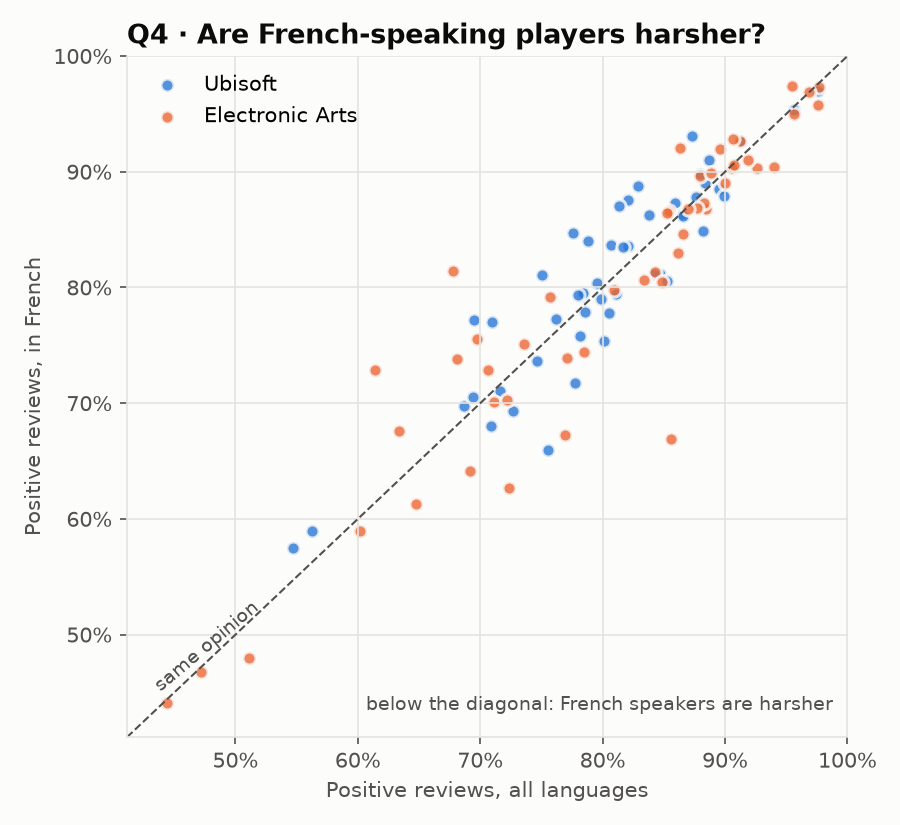
\includegraphics[width=0.6\linewidth]{q4_francophones.png}
\caption{Satisfaction in French and in all languages, per game}
\end{figure}

French speakers are slightly more generous, by +2.5 points towards EA and +2.1 towards Ubisoft. They are clearly more positive on
9 Ubisoft games and harsher on only 2. Yet they write only \textbf{2\% of reviews}.

\subsection{Recommendations to the client}
\begin{keybox}[For Lumen Forge Games]
\begin{enumerate}[leftmargin=1.4em]
  \item \textbf{Price:} €25 sits in a well-rated band. Raising the price raises expectations.
  \item \textbf{Launch is not a final verdict:} plan a patch roadmap. A reputation can recover.
  \item \textbf{Monitor reviews month by month:} a crisis can strike years after release.
  \item \textbf{Lifetime:} content updates or a co-op mode extend a game's life.
  \item \textbf{Market:} localise into French, but aim international, which drives Steam reputation.
\end{enumerate}
\end{keybox}

% =============================================================================
\section{Limitations and technical debt}\label{sec:limits}

\begin{tabularx}{\linewidth}{@{}L{5.2cm} Y@{}}
\toprule
\textbf{Limitation} & \textbf{Consequence} \\
\midrule
Steam only & Findings apply to Steam players, not other platforms \\
Snapshot (Wednesday, around 7 pm) & No seasonality. Discounts not measurable. \\
Current list price & Possible survivorship bias (Q2) \\
Years on Steam & Differs from actual age for re-released games (Q1b, Q3) \\
``French speakers'' = reviews in French & Country and native language are unknown \\
Correlation & Does not prove causation \\
\midrule
\multicolumn{2}{@{}l}{\textbf{Technical debt accepted at level 0}} \\
\midrule
No unit tests & Introduced in project 1 (\texttt{pytest}) \\
No scheduling & Manual runs. Orchestration planned for project 3. \\
Non-deterministic discovery & Reservation R1. Crawl the publisher's full catalogue. \\
Full refresh & No history between runs. Incremental loading planned for project 2. \\
\bottomrule
\end{tabularx}

% =============================================================================
\section{Lessons learned}
\begin{itemize}[leftmargin=1.2em]
  \item \textbf{Scope before coding:} a vague request became four measurable questions, each tied to a client decision.
  \item \textbf{Test APIs before promising:} the \texttt{day\_range} parameter does not do what its name suggests.
  \item \textbf{Distrust perfect results:} ``0 exclusions'' hid a traceability gap.
  \item \textbf{Design for failure:} thanks to the cache, an interruption was resolved within a minute.
  \item \textbf{State what the data cannot tell:} the discount question remains open, and the report says so.
\end{itemize}

% =============================================================================
\section{Roadmap}
\begin{tabularx}{\linewidth}{@{}L{4.3cm} Y@{}}
\toprule
\textbf{Improvement} & \textbf{Benefit} \\
\midrule
Tests and PostgreSQL & Robustness and a server database (portfolio project 1) \\
Daily incremental loading & Price history, seasonality, discounts (project 2) \\
Orchestration and dbt & Scheduling, \emph{bronze, silver, gold} layers (project 3) \\
Reputation alert & Notify when a month's share of positive reviews drops below a threshold \\
Panel of indie publishers & A comparison closer to the client's size \\
\bottomrule
\end{tabularx}

% =============================================================================
\appendix
\section{Data dictionary: \texttt{games} table}\label{app:dict}
\small
\begin{longtable}{@{}L{4.1cm} L{2.0cm} L{8.3cm}@{}}
\toprule
\textbf{Column} & \textbf{Type} & \textbf{Description} \\
\midrule\endhead
\texttt{app\_id} & INTEGER & Steam identifier of the game (primary key) \\
\texttt{name} & VARCHAR & Game title \\
\texttt{publisher\_group} & VARCHAR & Publisher analysed: Ubisoft or Electronic Arts \\
\texttt{publishers} / \texttt{developers} & VARCHAR & Publisher(s) and studio(s) declared on Steam \\
\texttt{is\_free} & BOOLEAN & Free-to-play game \\
\texttt{price\_initial\_eur} & DECIMAL & Current list price excluding discounts, in euros (not the launch price) \\
\texttt{price\_final\_eur} & DECIMAL & Price paid on extraction day \\
\texttt{discount\_percent} & INTEGER & Current discount (\%) \\
\texttt{steam\_release\_date} & DATE & Release date on Steam \\
\texttt{years\_on\_steam} & DECIMAL & Years on Steam at extraction date \\
\texttt{genres} & VARCHAR & Steam genres, in French \\
\texttt{metacritic\_score} & INTEGER & Press score, when available \\
\texttt{owners\_estimate\_low/high} & BIGINT & SteamSpy range of estimated owners \\
\texttt{extracted\_on} & DATE & Extraction date \\
\bottomrule
\end{longtable}
\normalsize
Full dictionary of the five tables: \texttt{docs/dictionnaire-de-donnees.md} (in French).

\section{Architecture decision records (ADR)}
\begin{tabularx}{\linewidth}{@{}l Y@{}}
\toprule
ADR 001 & Technology stack: DuckDB, pandas, \texttt{requests}, full refresh \\
ADR 002 & Extraction strategy: two passes, dated raw layer, cache, minimisation at the source \\
ADR 003 & Player count source: official Steam API rather than SteamSpy \\
\bottomrule
\end{tabularx}

\section{Repository structure}
\begin{lstlisting}[basicstyle=\ttfamily\footnotesize]
ubisoft-vs-ea-steam-etl/
|-- src/          extract.py, transform.py, load.py, report.py, pipeline.py, config.py
|-- sql/          00_schema.sql, q1a ... q4b (10 queries), controle_recette.sql
|-- docs/
|   |-- mission/      brief, scoping minutes, statement of work (French)
|   |-- decisions/    ADR 001 to 003
|   |-- journal/      dated work log
|   |-- livraison/    PDF reports, resultats.md, charts, acceptance sign-off
|   `-- rapport/      LaTeX sources of this report
|-- data/         raw batches and DuckDB database (not versioned, rebuilt by the pipeline)
|-- README.md  CHANGELOG.md  LICENSE  requirements.txt
\end{lstlisting}

\section{Glossary}
\begin{tabularx}{\linewidth}{@{}>{\bfseries}L{3.6cm} Y@{}}
ETL & Extract, Transform, Load \\
Raw layer & Data kept exactly as received from the sources, unchanged \\
Idempotency & Property of a process that gives the same result whether run once or several times \\
Full refresh & Complete replacement of the tables on every run \\
Atomic write & A write that either fully succeeds or does not happen at all \\
ADR & Architecture Decision Record: a short note tracing a technical decision and its rationale \\
Acceptance & Formal check, by the client, that the deliverable meets the agreed criteria \\
\emph{Review bombing} & Sudden, massive wave of negative reviews, often in reaction to a publisher decision \\
\end{tabularx}

\end{document}
